% Векторизация - целочисленный контекст.
\subsection{Векторизация целочисленного программного \\ контекста}

В разделах~\ref{sec:text_4_vec_riemann} и \ref{sec:text_4_vec_irreg} были рассмотрены подходы к векторизации\label{term:vectorization5} плоских циклов\label{term:flat_loop5} с телом в виде циклов с непостоянным количеством итераций.
В этих разделах входными данными рассматриваемой задачи являлись массивы вещественнных чисел.
В этом разделе будет рассмотрен пример векторизации для так называемого целочисленного программного контекста\label{term:integer_context}.
Под целочисленным программным контекстом будем подразумевать программный код, в котором преобладают целочисленные вычисления, а также ведется работа с дискретными структурами данных.

Рассмотренный в разделе~\ref{sec:text_2_genetic} алгоритм пузырькового роста\label{term:alg_decomp_bubble2}, используемый в генетическом алгоритме декомпозиции\label{term:alg_decomp_gen2} графа требует для своего применения эффективной реализации, так как в составе генетического алгоритма он должен исполняться многократно.
Этот алгоритм работает с целочисленным программным контекстом и может быть векторизован с помощью векторных операций над упакованными целыми числами.

\subsubsection{Скалярная реализация алгоритма пузырькового роста}

Рассмотрим возможности по ускорению алгоритма пузырьковго роста с помощью векторизации.
Пусть мы имеем граф, информация о его ребрах записана в структуре \texttt{vector<vector<int>> inc}, где \texttt{inc[i]} –- список номеров всех вершин, смежных с вершиной $i$.
Номера доменов, к которым относятся конкретные вершины хранятся в структуре \texttt{vector<int> domains}.
Структура \texttt{vector<queue<int>> q} -– список очередей вершин, ожидающих попадания в домены, в начале работы алгоритма очередь \texttt{q[i]} содержит только одну инициирующую вершину $i$-го домена.
Пусть требуется выполнить декомпозицию (или раскраску графа) на \texttt{domains\_count} доменов.
Тогда реализация алгоритма пузырькового роста доменов от инициирующих вершин может иметь следующий вид (см. листинг~\ref{lst:text_4_vec_integer}):

\begin{lstlisting}[caption={Реализация алгоритма пузырькового роста доменов.},label={lst:text_4_vec_integer}]
while (is_q)
{
    is_q = false;

    for (size_t c = 0; c < domains_count; ++c)
    {
        if (q[c].empty()) continue;

        is_q = true;
        n = q[c].front();
        q[c].pop();

        if (domains[n] == -1)
        {
            domains[n] = c;
            for (auto ngh : inc[n]) q[c].push(ngh);
        }
    }
}
\end{lstlisting}

Реализация алгоритма представляет собой гнездо из 3 циклов.
Внешний цикл выполняется до тех пор, пока найдется хотя бы одна непустая очередь домена.
Средний цикл выполнятся по номерам доменов.
Для каждого домена берется первая необработанная вершина из соответствующей очереди, и если она еще не отнесена ни к одному домену, то она заносится в текущий домен, а все ее соседи отправляются в очередь.
Внутренний цикл -– цикл по всем соседям только что обработанной вершины, которые должны быть занесены в очередь.
Будем выполнять векторизацию представленного кода по среднему циклу, и для простоты анализа приведем реализацию для фиксированного значения \texttt{domains\_count = 16} (это позволит избавиться от среднего цикла, и заменить его набором отдельных векторных операций).

Для выполнения векторизации вначале необходимо избавиться от STL структур \texttt{vector}  и \texttt{queue}, так как они имеют свою внутреннюю реализацию, и векторизация операций по работе с ними невозможна.
Вместо структуры \texttt{vector<int>} будем хранить информацию о списке соседних вершин просто в массиве, 0-м элементом которого будет его размер.
Очередь \texttt{queue} также будет имитировать с помощью массива и индексов \texttt{front} и \texttt{back}, указывающих на первый и последний элементы очереди соответственно.
Тогда операция \texttt{push(v)} будет соответствовать записи в массив по индексу \texttt{back} с его продвижением, а операция \texttt{pop} будет соответствовать просто продвижению индекса \texttt{front}.
Очередь пуста если ее индекс \texttt{front} больше индекса \texttt{back}.

\subsubsection{Векторная реализация алгоритма пузырькового роста}

\begin{figure}[ht]
\centering
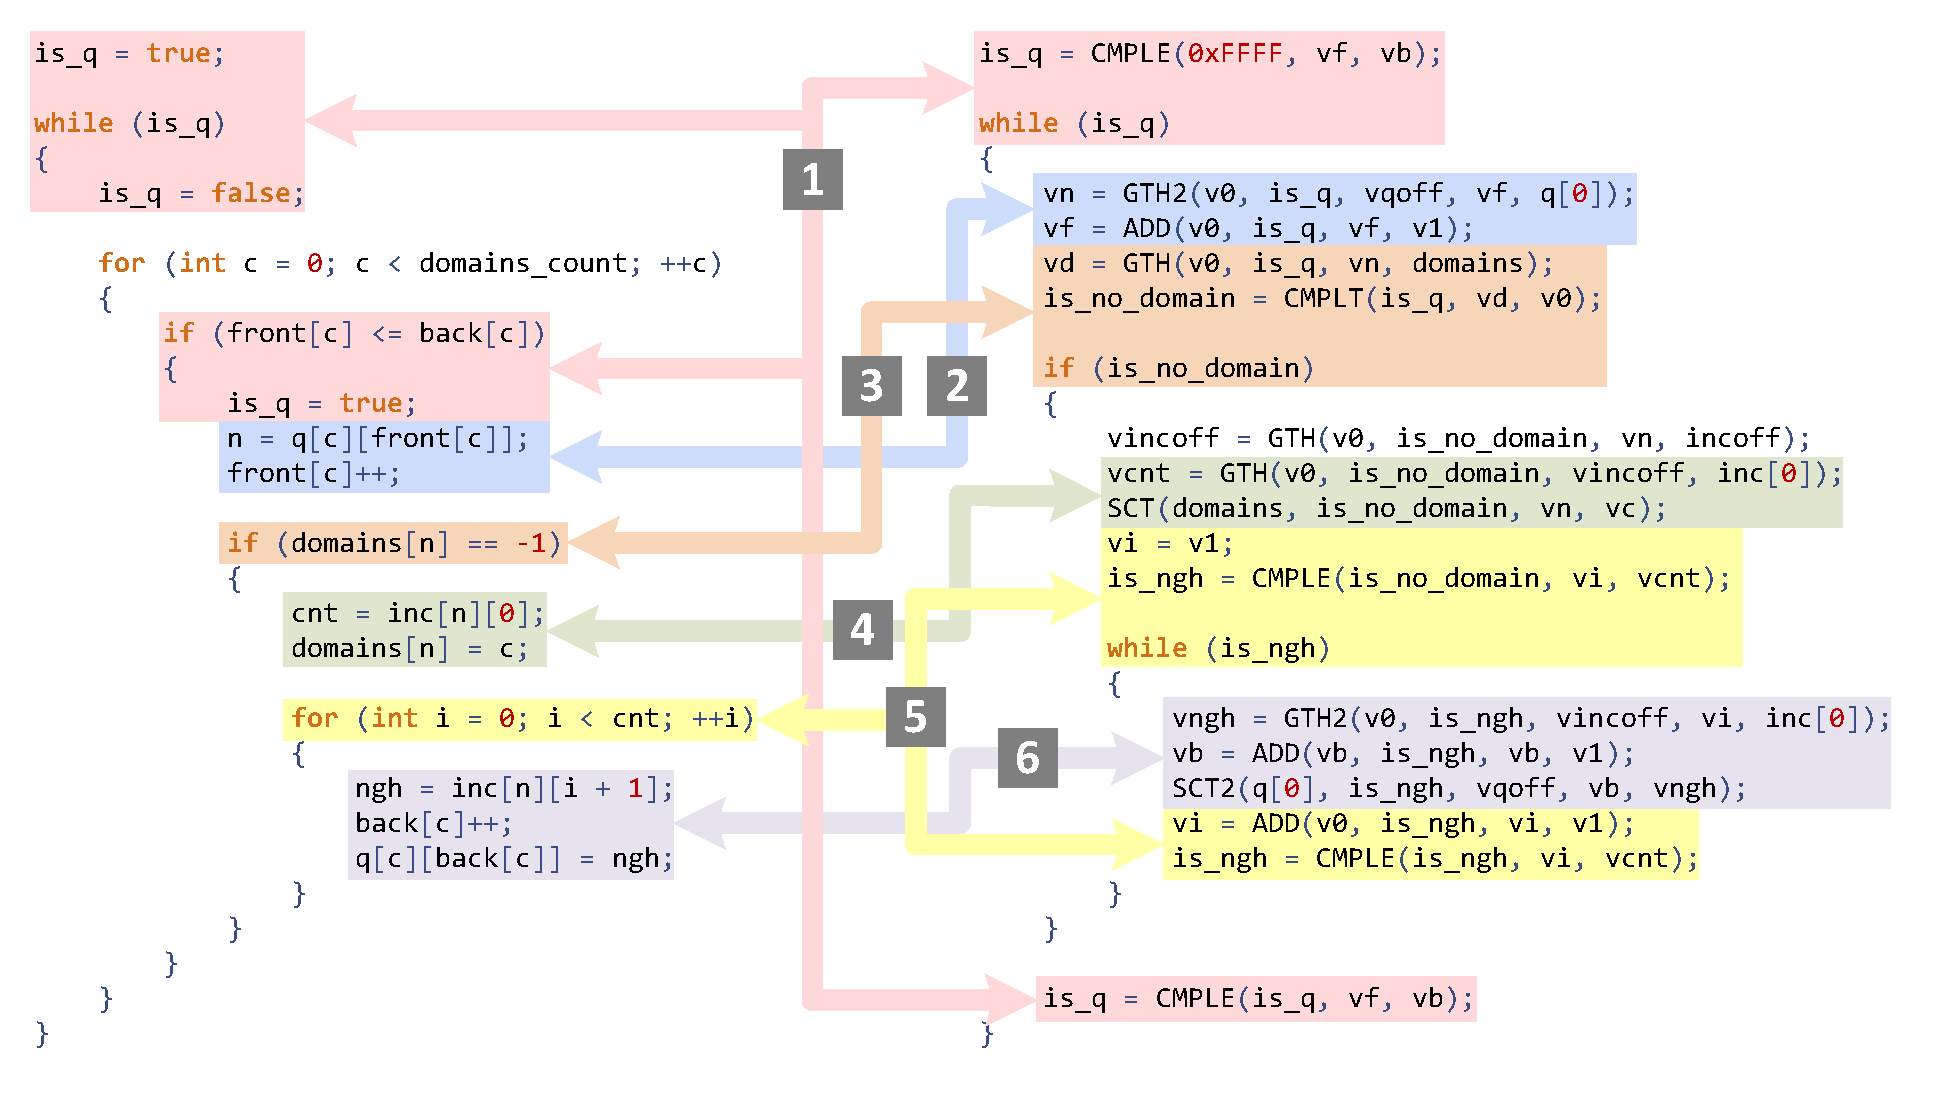
\includegraphics[width=1.0\textwidth]{pics/text_4_vec_integer/code.pdf}
\singlespacing
\captionstyle{center}\caption{Векторизация программного кода алгоритма пузырькового роста путем замены скалярных инструкций векторными аналогами.}
\label{fig:text_4_vec_integer_code}
\end{figure}

На рис.~\ref{fig:text_4_vec_integer_code} представлены скалярная и векторная версии программного кода реализации алгоритма пузырькового роста.
Полная версия исходного кода доступна в \cite{comboptGithub}.
В векторной версии через \texttt{ADD}, \texttt{GTH}, \texttt{SCT} обозначаются функции-интринсики \texttt{\_mm512\_mask\_add\_epi32}, \texttt{\_mm512\_mask\_i32gather\_epi32}, \texttt{\_mm512\_mask\_i32scatter\_epi32} соответственно (\texttt{GTH2} и \texttt{SCT2} это те же операции \texttt{GTH} и \texttt{SCT}, только использующие сразу два смещения от базового адреса).
Через \texttt{CMPLE}, \texttt{CMPLT} обозначены вызовы функции-интринсика \texttt{\_mm512\_mask\_cmp\_epi32\_mask} с параметрами сравнения \texttt{\_MM\_CMPINT\_LE} и \texttt{\_MM\_CMPINT\_LT} соответственно.
На рис.~\ref{fig:text_4_vec_integer_code} цифрой <<1>> обозначена векторизация условия продолжения выполнения внешнего цикла (цикл завершает работу, если все очереди доменов пусты).
Цифрой <<2>> обозначена векторизация извлечения следующей вершины из каждой очереди.
Цифрой <<3>> обозначена проверка принадлежности извлеченных вершин к какому-либо домену (в векторной версии формируется маска \texttt{is\_no\_domain} -- маска с номерами доменов, в которые добавляется новая вершина).
Цифрой <<4>> обозначена векторизация помещения рассматриваемой вершины в текущий домен и получение количества ее соседей. 
Цифра <<5>> -- обработка всех соседей только что помещенной в домен вершины, и цифра <<6>> -- добавление этих соседей в соответствующие очереди.

Стоит отметить, что векторизованная версия представленного алгоритма не является полностью эквивалентной скалярной версии. 
Вполне может оказаться, что на какой-то итерации внешнего цикла из двух или более разных очередей одновременно будет извлечена одна и та же вершина.
В этом случае в векторной версии она будет отнесена к домену с наибольшим номером (хотя в скалярном аналоге, она бы попала в домен с меньшим номером).
Это несоответствие можно устранить путем разворачивания векторов \texttt{vn} и \texttt{vc} при записи в массив \texttt{domains} (цифра «4» на рис.~\ref{fig:text_4_vec_integer_code}), но это не делалось, чтобы не усложнять код.

\subsubsection{Оценка эффективности векторизации алгоритма пузырькового роста}

Для оценки эффективности проведенной векторизации были произведены запуски на дуальных графах поверхностных прямоугольных расчетных сеток со стороной от 20 до 2000 ячеек (то есть на графах с количеством вершин от 400 до 4 млн).
На рис.~\ref{fig:text_4_vec_integer_stat} представлена собранная статистика плотности масок (доля выставленных битов) векторных операций различных типов.
Из графиков на рис.~\ref{fig:text_4_vec_integer_stat} можно сразу сделать вывод о невысокой эффективности векторизации, так как плотность масок арифметических операций и операций записи в память оказались довольно низкими (примерно 0,3 и 0,25 соответственно).

\begin{figure}[ht]
\centering
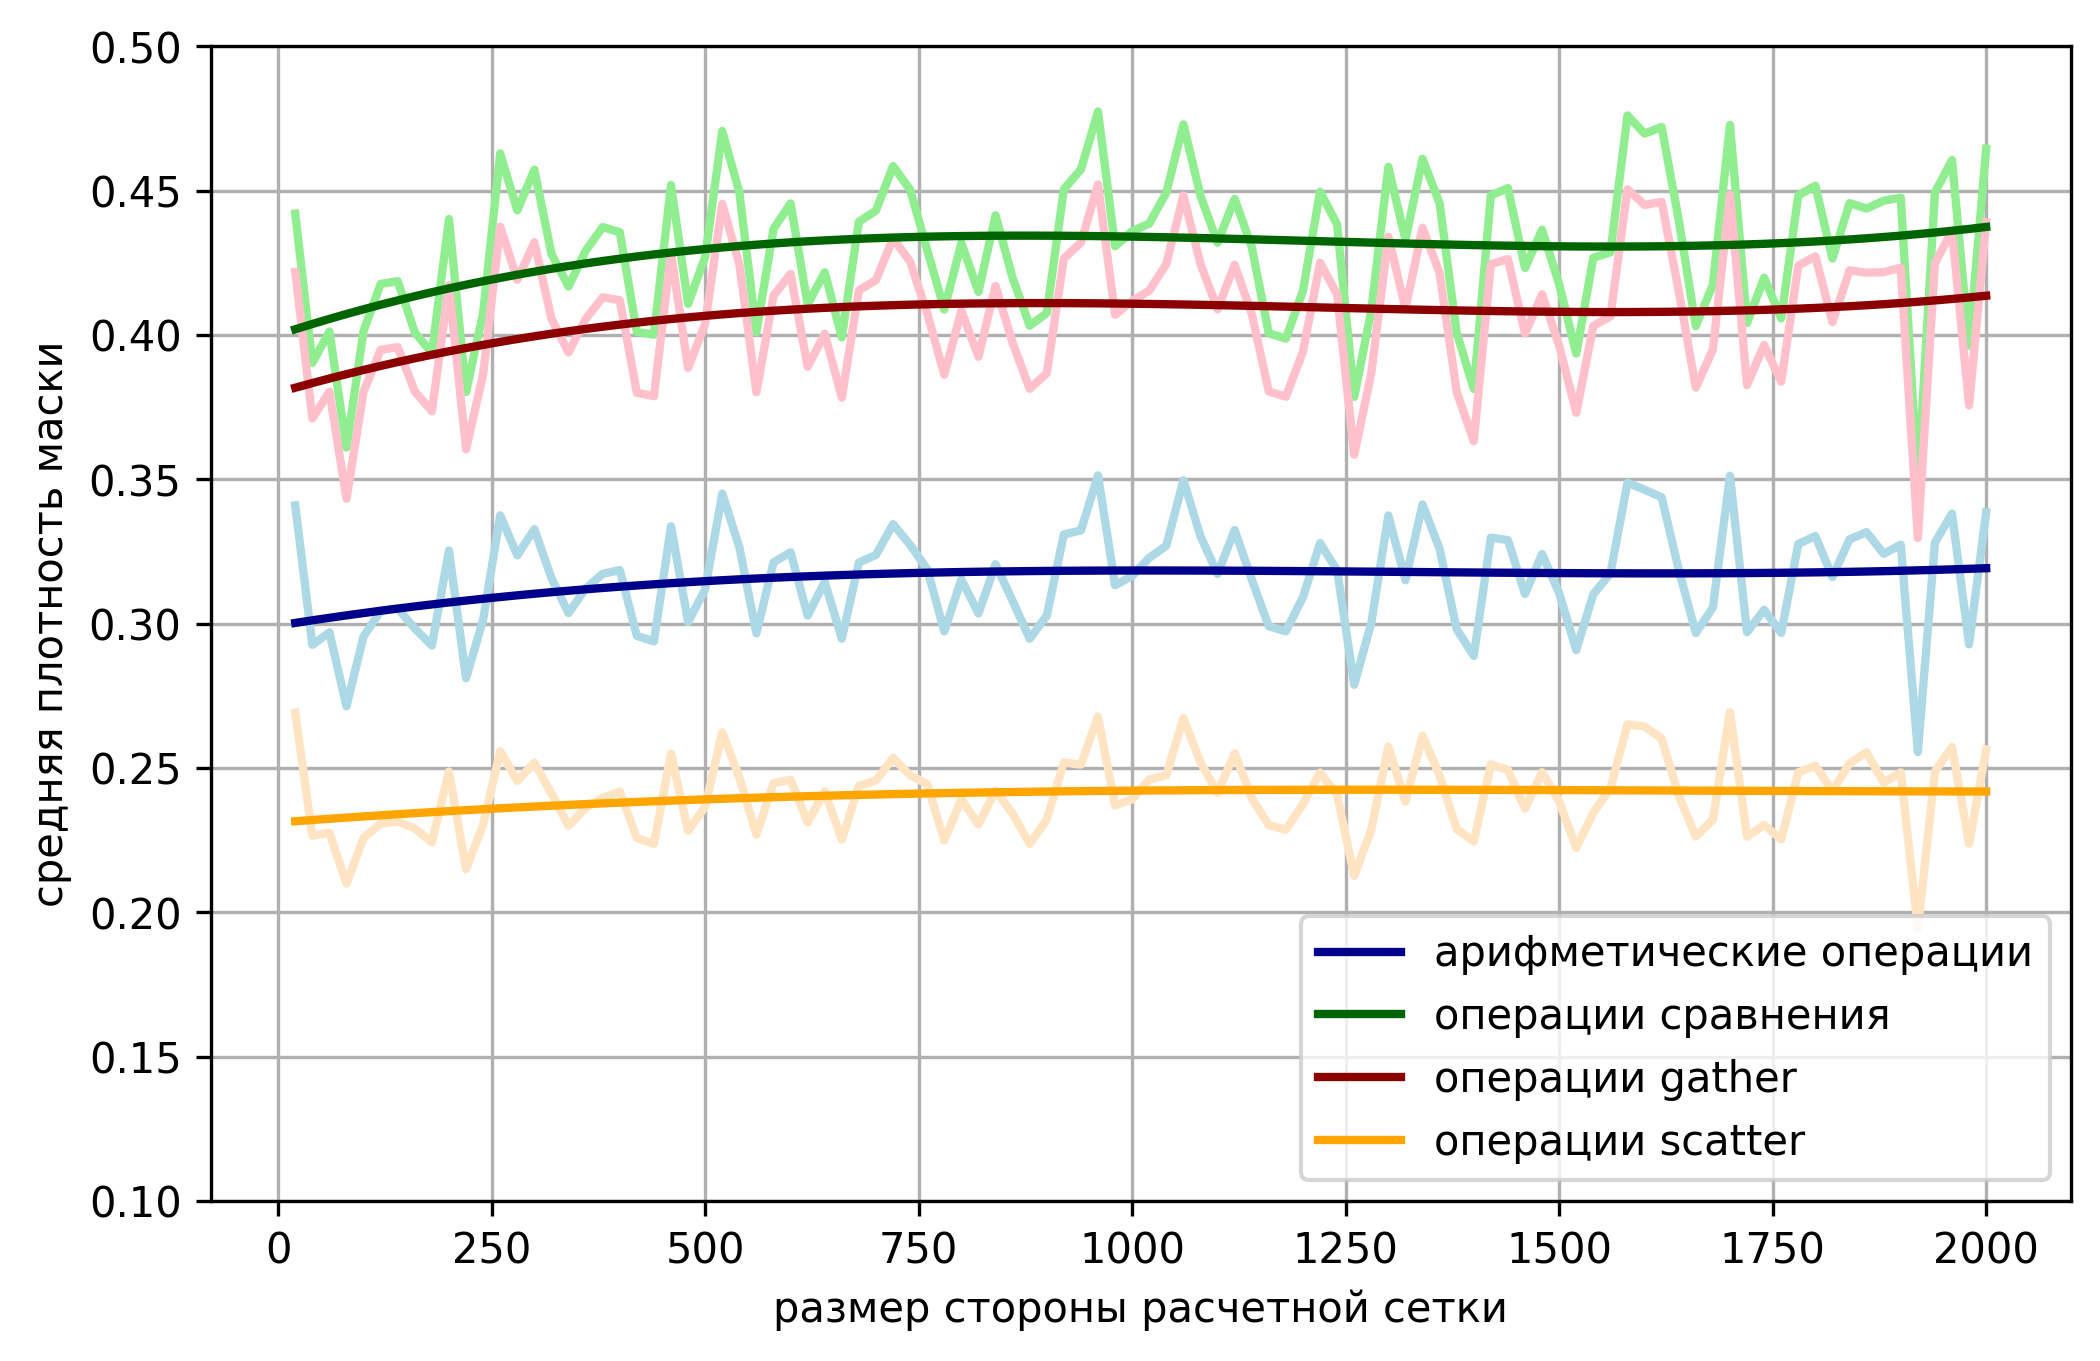
\includegraphics[width=0.8\textwidth]{pics/text_4_vec_integer/chart_statistics_rus.png}
\singlespacing
\captionstyle{center}\caption{Средняя плотность масок разных классов операций AVX-512 в зависимости от размера стороны расчетной сетки.}
\label{fig:text_4_vec_integer_stat}
\end{figure}

Замеры реального ускорения выполнялись для тех же графов на микропроцессоре Intel Xeon Phi 7290, результаты представлены на рис.~\ref{fig:text_4_vec_integer_sp}, для удобства приведен также график сглаженного показателя ускорения.
Анализирую график сглаженного показателя ускорения, можно отметить, что максимум наблюдается при размере стороны расчетной сетки в районе 750 и равен при мерно 1,95.
Снижение ускорения при уменьшении стороны расчетной сетки связано с увеличение количества конфликтов при обработке следующих вершин из очередей доменов.
Снижение ускорения при увеличении стороны расчетной сетки связано с увеличением разброса смещений при выполнении операций gather/scatter, что приводит к промахам в кэш-память.

\begin{figure}[ht]
\centering
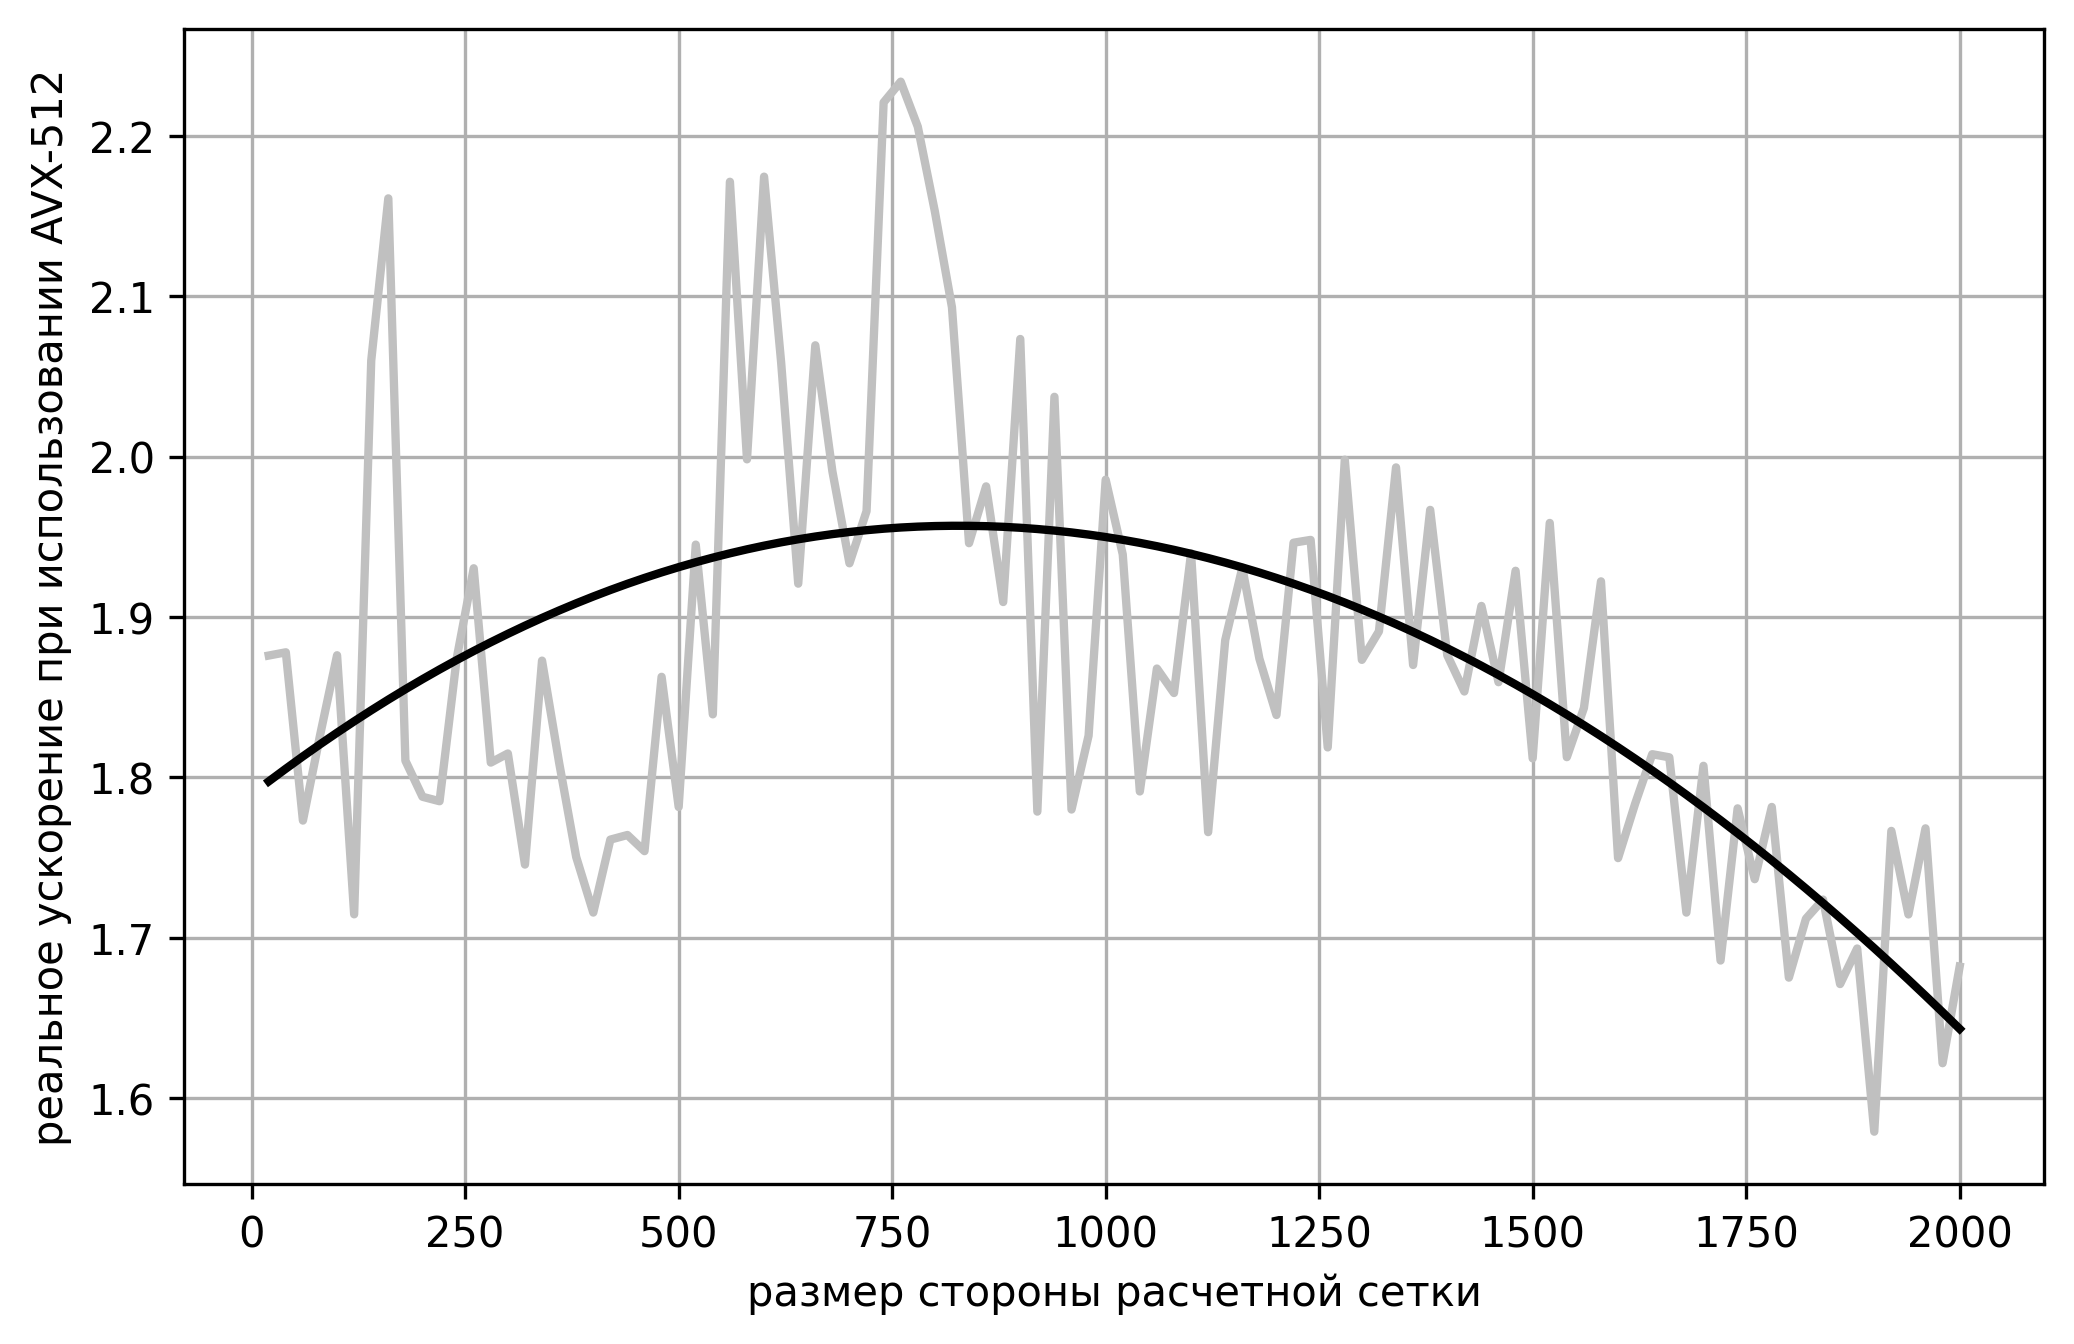
\includegraphics[width=1.0\textwidth]{pics/text_4_vec_integer/chart_speedup_rus.png}
\singlespacing
\captionstyle{center}\caption{Ускорение вычислений в зависимости от размера стороны расчетной сетки, полученное при запусках на микропроцессоре Intel Xeon KNL 7290.}
\label{fig:text_4_vec_integer_sp}
\end{figure}

В разделе рассмотрен алгоритм пузырькового роста, используемый для декомпозиции графа.
Этот алгоритм применяется для выполнения декомпозиции как в роли самостоятельного метода, так и в составе других, более комплексных подходов к декомпозиции.
Была рассмотрена реализация, в которой для каждого домена поддерживается своя очередь обрабатываемых вершин графа.
Такой подход допускает одновременную обработку очередей доменов, что делает возможным применение векторизации для ускорения вычислений.
Был предложен вариант векторизации алгоритма по среднему циклу гнезда для фиксированного количества доменов, равного 16.
Для полученного варианта векторизации была собрана статистика плотности векторных масок векторных операций в результирующем коде, которая показала крайне низкие значения для арифметических операций (около 0,3) и операций записи в память (около 0,25). 
Замеры ускорения на микропроцессоре Intel Xeon Phi 7290 продемонстрировали ускорение в диапазоне 1,7-2,2 раза для рассматриваемых графов с количеством ячеек от 400 до 4 млн.
Такие невысокие результаты ускорения объясняются прежде всего нерегулярным количеством итераций циклов в гнезде, а также обилием операций множественного обращения в память gather/scatter.
